Ein Ball wird mit \vNullO\ senkrecht nach oben geworfen und auf derselben Höhe wieder aufgefangen. Die Luftreibung ist vernachlässigbar. Mit der positiven Richtung nach oben nimmt seine Geschwindigkeit gleichmässig ab, von $+v_0$ bis $-v_0$ beim Auffangen (zur Zeit $t_\mathrm{L}$):
\begin{center}
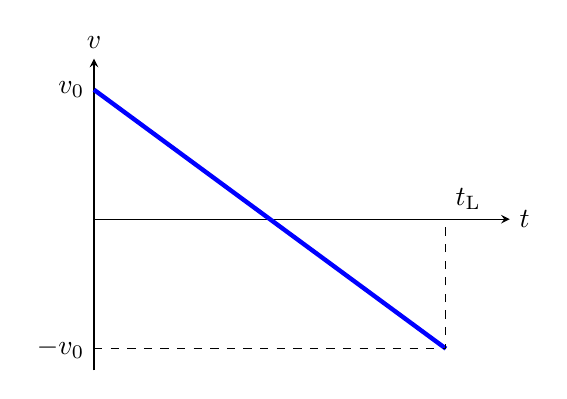
\begin{tikzpicture}[>=stealth, x=1.6cm, y=0.12cm]
 \draw[->] (0,0) -- (3.3,0) node[right] {$t$};
 \draw[->] (0,-16) -- (0,17) node[above] {$v$};
 \draw[ultra thick, blue] (0,13.7) -- (2.793,-13.7);
 \draw[dashed] (0,-13.7) -- (2.793,-13.7) -- (2.793,0);
 \node[left] at (0,13.7) {$v_0$};
 \node[left] at (0,-13.7) {$-v_0$};
 \node[above right] at (2.793,0) {$t_\mathrm{L}$};
\end{tikzpicture}
\end{center}
\begin{abcliste}
\abc Wann wird der Ball aufgefangen?
\abc Wo ist der Ball zur Zeit $t_\mathrm{L}$, verglichen mit dem Abwurfort? Begründen Sie mit dem $v(t)$-Diagramm.
\abc Welche Strecke legt der Ball insgesamt zurück?
\end{abcliste}
